\documentclass[10pt, aspectratio=169]{beamer}

% --- Configuración del Tema ---
\usetheme{metropolis}
\usecolortheme{owl} 
\usepackage[spanish]{babel}
\usepackage[utf8]{inputenc}
\usepackage{amsfonts, amsmath, amssymb, amsthm}
\usepackage{graphicx}
\usepackage{tikz}

% --- Colores Personalizados ---
\definecolor{diagonalred}{RGB}{140, 20, 40}

% --- Información del Título ---
\title{Los Límites de la Razón}
\subtitle{Sesión 4: El Logicismo, Peano y la Caída de los Dioses}
\author{Rosh Guadiana}
\date{Junio 2026}

\begin{document}

\maketitle

% ==========================================
% EL LOGICISMO
% ==========================================

\begin{frame}{El Logicismo: Principia Mathematica}
    \vspace{0.4cm}
    \Large \textbf{El sueño de Russell y Whitehead}
    
    \vspace{0.4cm}
    \normalsize
    Un programa fundacional para demostrar que \textbf{toda la matemática es solo un capítulo maduro de la lógica pura}. 
    
    \vspace{0.6cm}
    \alert{\textbf{El objetivo:}} \\
    Definir todas las nociones aritméticas (números, sumas, orden) usando únicamente ideas lógicas (conjuntos, cuantificadores) y deducir la aritmética mediante proposiciones puramente lógicas.
\end{frame}

\begin{frame}{El Fracaso del Isomorfismo}
    \vspace{0.3cm}
    \Large \textbf{El traslado de la carga}
    
    \vspace{0.4cm}
    \normalsize
    La idea era brillante: si logramos un isomorfismo perfecto entre aritmética y lógica, entonces \textbf{si la lógica es consistente, la aritmética también lo es}.
    
    \vspace{0.6cm}
    \alert{\textbf{¿Resolvió esto el problema? No.}} \\
    Simplemente lo generalizó. La pregunta pasó de ``¿Es la aritmética consistente?'' a ``¿Estamos seguros de que nuestro vasto sistema lógico está libre de contradicciones?''. Había que volver a la base.
\end{frame}

% ==========================================
% LA ARITMÉTICA DE PEANO
% ==========================================

\begin{frame}{La Firma de Peano}
    \vspace{0.3cm}
    \Large \textbf{Definimos: ($\mathcal{L}_{PA}$)}
    
    \vspace{0.6cm}
    \normalsize
    \begin{columns}
        \begin{column}{0.5\textwidth}
            \alert{\textbf{Símbolos de Función ($\mathcal{F}$):}}
            \large
            \begin{itemize}
                \item Constante: $0$ ($ar=0$)
                \item Sucesor: $S$ ($ar=1$)
                \item Operadores: $+, \cdot$ ($ar=2$)
            \end{itemize}
        \end{column}
        \begin{column}{0.5\textwidth}
            \alert{\textbf{Símbolos de Predicado ($\mathcal{P}$):}}
            \large
            \begin{itemize}
                \item Igualdad: $=$ ($ar=2$)
            \end{itemize}
        \end{column}
    \end{columns}
\end{frame}

\begin{frame}{Los Axiomas de Peano ($PA$)}
    \vspace{0.2cm}
    \small \textbf{Definición mecánica de los números naturales:}

    
    \vspace{0.2cm}
    \footnotesize
    \begin{itemize}
        \setlength\itemsep{0.3cm}
        \item \textbf{Cero y Sucesor:} 
        $$PA_1: \forall x \, (S(x) \neq 0) \quad \quad PA_2: \forall x \forall y \, (S(x) = S(y) \to x = y)$$
        
        \item \textbf{La Suma Recursiva:}
        $$PA_3: \forall x \, (x + 0 = x) \quad \quad PA_4: \forall x \forall y \, (x + S(y) = S(x + y))$$
        
        \item \textbf{El Producto Recursivo:}
        $$PA_5: \forall x \, (x \cdot 0 = 0) \quad \quad PA_6: \forall x \forall y \, (x \cdot S(y) = (x \cdot y) + x)$$
        
        \item \textbf{Esquema de Inducción:}
        $$PA_7: (\phi(0) \land \forall x \, (\phi(x) \to \phi(S(x)))) \to \forall x \, \phi(x)$$
    \end{itemize}
\end{frame}
% ==========================================
% SUSTITUCIÓN Y TERCERO EXCLUIDO
% ==========================================

\begin{frame}{El Principio de Sustitución (\textit{Salva Veritate})}
    \begin{definicion}[Sustitución de los Idénticos]
        Atribuido a Leibniz, el principio establece que si dos términos designan al mismo objeto, uno puede ser sustituido por el otro en cualquier fórmula lógica sin alterar su valor de verdad (\textit{salva veritate}).
    \end{definicion}

    \vspace{0.6cm}
    \Large \textbf{Formalización en LPO}
    
    \vspace{0.4cm}
    \normalsize
    Sea $\phi(x)$ una fórmula con la variable libre $x$. El esquema axiomático de sustitución para el predicado de igualdad dicta estrictamente:
    
    \vspace{0.4cm}
    \huge
    $$\vdash \forall x \forall y \, \Big( x = y \to \big( \phi(x) \leftrightarrow \phi(y) \big) \Big)$$
\end{frame}

\begin{frame}{Ejemplo}
    \vspace{2.5cm}
    \begin{center}
        \Huge \textbf{Primos Infinitos}
    \end{center}
\end{frame}
% ==========================================
% LIMITACIONES SEMÁNTICAS vs SINTÁCTICAS
% ==========================================

\begin{frame}{El Espejismo Semántico}
    \begin{center}
        \Large \textbf{La Paradoja del Mentiroso}
        
        \vspace{1.0cm}
        \huge \textit{``Este enunciado no es verdad.''}
        \vspace{1.0cm}
    \end{center}
    
    \normalsize
    \alert{\textbf{Por qué es inútil matemáticamente:}} \\
    Juega con el concepto de ``verdad'', el cual es semántico y requiere interpretación humana. Las máquinas sintácticas (como $PA$) son ciegas; no tienen un detector de ``verdad'', solo aplican reglas de inferencia.
\end{frame}

\begin{frame}{El Giro Sintáctico de Gödel}
    \begin{center}
        \Large \textbf{El arma que destruyó el absolutismo}
        
        \vspace{1.0cm}
        \huge \textit{``Este enunciado no es \textbf{demostrable}.''}
        \vspace{1.0cm}
    \end{center}
    
    \normalsize
    \alert{\textbf{El genio absoluto:}} \\
    Gödel cambió ``verdad'' (semántica abstracta) por ``demostrabilidad'' (sintaxis mecánica pura). La máquina sí entiende la demostrabilidad, porque se reduce a verificar si existe una cadena válida de símbolos que conecte los axiomas.
\end{frame}

% ==========================================
% LA DIAGONALIZACIÓN Y LA ARITMETIZACIÓN
% ==========================================

\begin{frame}{La Matriz de Cantor (1891)}
    \begin{center}
        \Large \textbf{La diagonalización fundacional}
        
        \vspace{0.2cm}
        \begin{tikzpicture}[scale=1]
            % Matriz infinita
            \node at (0,4) {$s_1 = $}; \node at (1,4) {\textbf{\color{diagonalred}0}}; \node at (2,4) {$0$}; \node at (3,4) {$0$}; \node at (4,4) {$0$}; \node at (5,4) {$\dots$};
            \node at (0,3) {$s_2 = $}; \node at (1,3) {$1$}; \node at (2,3) {\textbf{\color{diagonalred}1}}; \node at (3,3) {$1$}; \node at (4,3) {$1$}; \node at (5,3) {$\dots$};
            \node at (0,2) {$s_3 = $}; \node at (1,2) {$0$}; \node at (2,2) {$1$}; \node at (3,2) {\textbf{\color{diagonalred}0}}; \node at (4,2) {$1$}; \node at (5,2) {$\dots$};
            \node at (0,1) {$s_4 = $}; \node at (1,1) {$1$}; \node at (2,1) {$0$}; \node at (3,1) {$0$}; \node at (4,1) {\textbf{\color{diagonalred}1}}; \node at (5,1) {$\dots$};
            \node at (0,0) {$\vdots$}; \node at (1,0) {$\vdots$}; \node at (2,0) {$\vdots$}; \node at (3,0) {$\vdots$}; \node at (4,0) {$\vdots$}; \node at (5,0) {$\ddots$};
            
            % Highlight de la diagonal
            \draw[diagonalred, thick, rounded corners] (0.6, 4.4) -- (1.4, 4.4) -- (4.4, 0.6) -- (3.6, 0.6) -- cycle;
            
            % El nuevo número
            \node at (7, 2.5) {\Large $s^* = $};
            \node at (8, 2.5) {\textbf{\color{diagonalred}1}};
            \node at (8.5, 2.5) {\textbf{\color{diagonalred}0}};
            \node at (9, 2.5) {\textbf{\color{diagonalred}1}};
            \node at (9.5, 2.5) {\textbf{\color{diagonalred}0}};
            \node at (10, 2.5) {$\dots$};
        \end{tikzpicture}
        
        \vspace{0.4cm}
    \end{center}
\end{frame}

\begin{frame}{El Arquitecto del Colapso: Kurt Gödel}
    \begin{columns}
        \begin{column}{0.4\textwidth}
            \begin{center}
                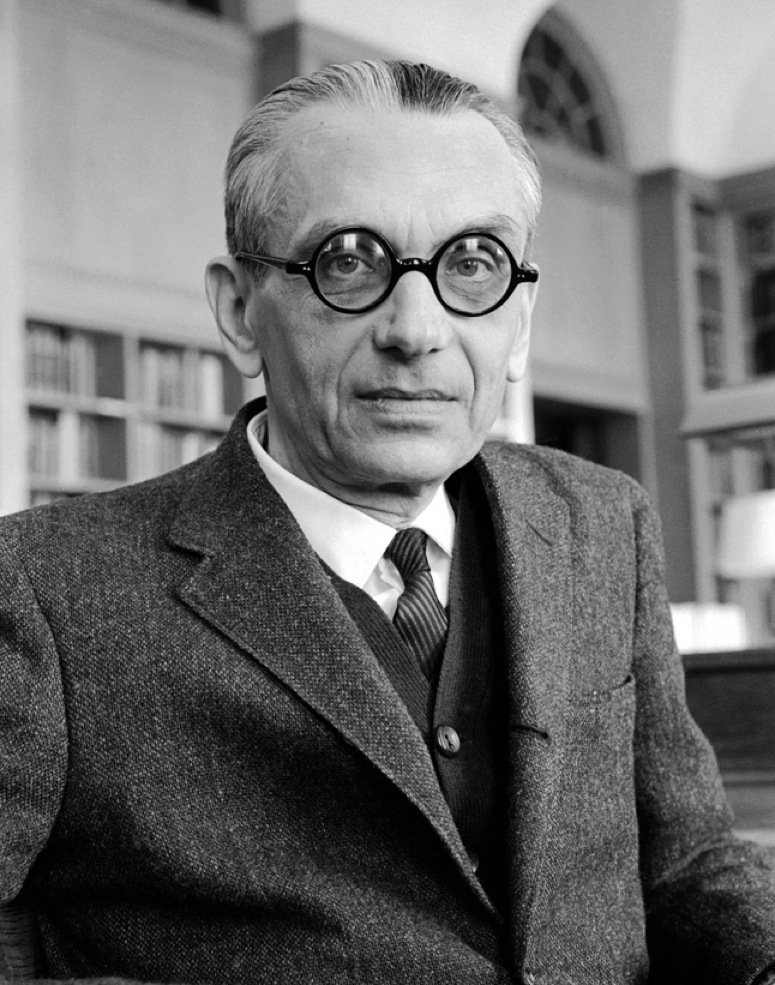
\includegraphics[height=0.75\textheight]{../../assets/Kurt-Godel.jpg} \\
                \vspace{0.2cm}
                \textbf{Kurt Gödel} \\
                \small (1906 -- 1978)
            \end{center}
        \end{column}
        \begin{column}{0.6\textwidth}
            \vspace{0.5cm}
            \Large \textbf{Aritmetización de la Sintaxis}
            
            \vspace{0.4cm}
            \normalsize
            Descubrió un isomorfismo inyectivo para incrustar el álgebra de la sintaxis lógica dentro del tejido de la aritmética pura.
            
            \vspace{0.4cm}
            \alert{\textbf{La herramienta clave:}} \\
            La unicidad de la factorización prima garantizada por el \textbf{Teorema Fundamental de la Aritmética}.
        \end{column}
    \end{columns}
\end{frame}

\begin{frame}{El ADN de la Máquina: Números de Gödel}
    \vspace{0.3cm}
    Una secuencia de símbolos (fórmula) $\phi = s_{i_1} s_{i_2} \dots s_{i_k}$ se convierte en un único entero colosal mediante:
    
    \vspace{0.6cm}
    \huge
    $$\ulcorner \phi \urcorner = 2^{c(s_{i_1})} \cdot 3^{c(s_{i_2})} \cdot 5^{c(s_{i_3})} \cdots p_k^{c(s_{i_k})}$$
    
    \vspace{0.6cm}
    \normalsize
    \begin{center}
        Donde $p_k$ representa el $k$-ésimo número primo absoluto.
    \end{center}
\end{frame}

\begin{frame}{Metáfora: Biología Matemática}
    \vspace{0.5cm}
    \Large \alert{\textbf{La Autoconsciencia del Número}}
    
    \vspace{0.6cm}
    \normalsize
    Así como las secuencias de nucleótidos (A, T, C, G) se combinan para codificar las instrucciones de un organismo complejo dentro de una molécula química...
    
    \vspace{0.6cm}
    \textbf{Gödel incrustó la estructura del pensamiento lógico dentro del cuerpo de los números primos.} Hizo que la aritmética adquiriera las herramientas para hablar de sí misma.
\end{frame}

% ==========================================
% LOS TEOREMAS DE INCOMPLETITUD
% ==========================================

\begin{frame}{El Punto Fijo y la Oración $G$}
    \vspace{0.3cm}
    Apoyándose en el \textbf{Lema Diagonal}, Gödel forzó la existencia de un punto fijo sintáctico para el predicado de demostrabilidad $\text{Prov}_{PA}(x)$:
    
    \vspace{0.6cm}
    \huge
    $$PA \vdash G \leftrightarrow \neg \text{Prov}_{PA}(\ulcorner G \urcorner)$$
    
    \vspace{0.6cm}
    \normalsize
    \begin{center}
        \textit{``Existe un número de Gödel equivalente a una secuencia de deducciones válidas que demuestra mi propio código.''} -- \textbf{FALSO.}
    \end{center}
\end{frame}

\begin{frame}{El Primer Teorema de Incompletitud (1931)}
    \vspace{0.4cm}
    \Large \textbf{El límite ineludible}
    
    \vspace{0.6cm}
    \normalsize
    Para cualquier sistema formal axiomático $F$ recursivamente enumerable y lo suficientemente fuerte como para describir la aritmética elemental (como $PA$):
    
    \vspace{0.6cm}
    \begin{center}
        \alert{\Large \textbf{Si $F$ es consistente, entonces $F$ es incompleto.}}
    \end{center}
    
    \vspace{0.6cm}
    \begin{center}
        \small Existen enunciados aritméticos verdaderos (como $G$) que el sistema no puede demostrar ni refutar. Verdad $\neq$ Demostrabilidad.
    \end{center}
\end{frame}

\begin{frame}{El Choque de Titanes: Hilbert vs. Von Neumann}
    \begin{columns}
        % Izquierda: La Soberbia
        \begin{column}{0.3\textwidth}
            \begin{center}
                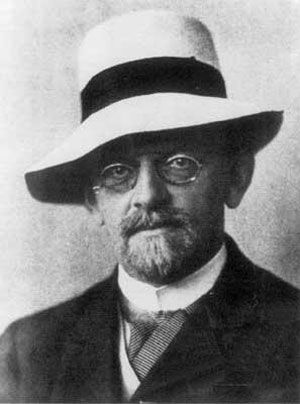
\includegraphics[height=0.45\textheight]{../../assets/David-Hilbert.jpg} \\
                \vspace{0.2cm}
                \textbf{David Hilbert} \\
                \vspace{0.1cm}
                \footnotesize \textit{\color{diagonalred} ``Wir müssen wissen, \\ wir werden wissen.''}
            \end{center}
        \end{column}
        
        % Centro: El Colapso Metamatemático
        \begin{column}{0.4\textwidth}
            \begin{center}
                \small \textbf{El sueño de Hilbert:} \\
                \vspace{0.1cm}
                $PA \vdash \text{Con}(PA)$
                
                \vspace{0.4cm}
                \small \textbf{Deducción de Von Neumann:} \\
                \vspace{0.1cm}
                $PA \vdash \big( \text{Con}(PA) \to G \big)$
                
                \vspace{0.4cm}
                \alert{\textbf{El Golpe Fatal:}} \\
                \footnotesize (Modus Tollens sobre el Primer Teorema) \\
                \vspace{0.2cm}
                \Large $PA \not\vdash \text{Con}(PA)$
            \end{center}
        \end{column}
        
        % Derecha: La Realidad
        \begin{column}{0.3\textwidth}
            \begin{center}
                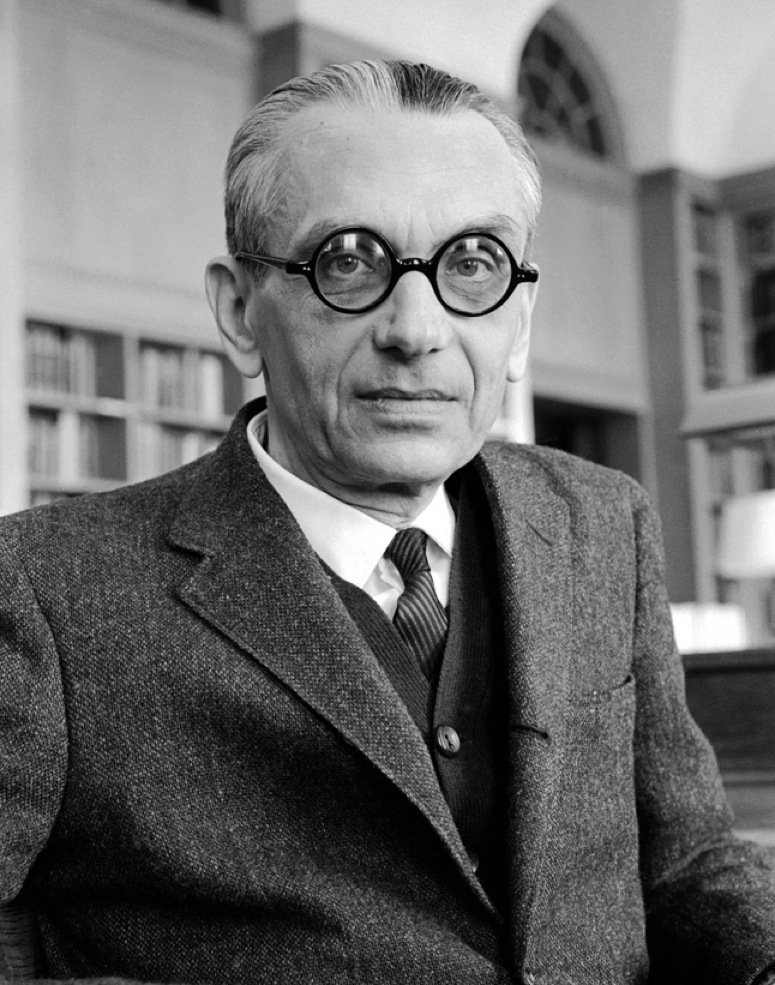
\includegraphics[height=0.3\textheight]{../../assets/Kurt-Godel.jpg} \\
                \vspace{0.1cm}
                \footnotesize \textbf{Kurt Gödel}
                
                \vspace{0.3cm}
                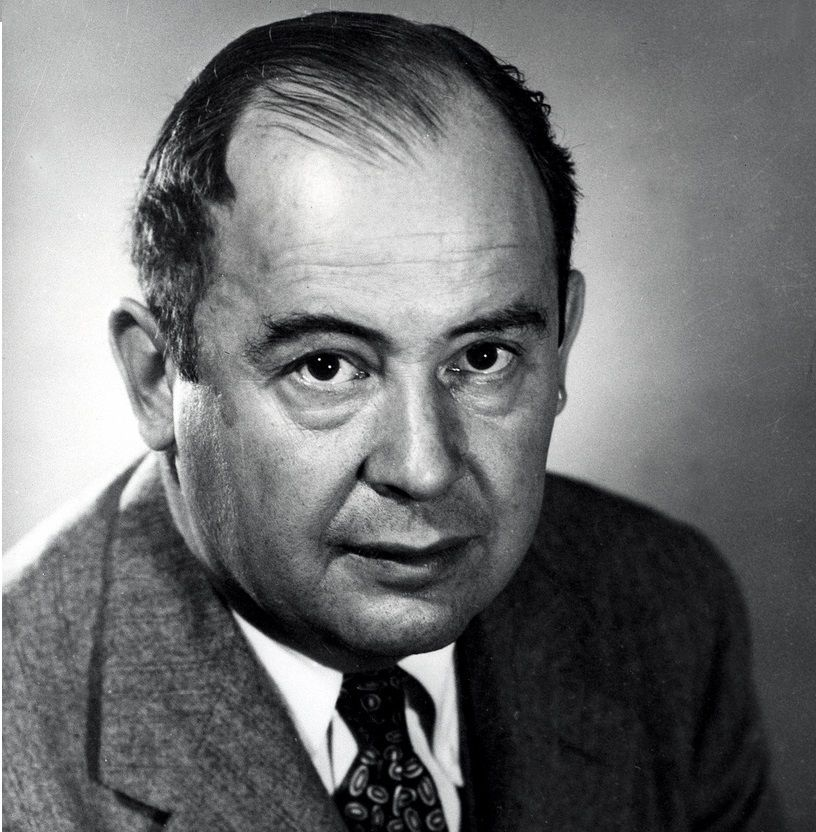
\includegraphics[height=0.3\textheight]{../../assets/John-von-Neumann.jpg} \\
                \vspace{0.1cm}
                \footnotesize \textbf{John von Neumann}
            \end{center}
        \end{column}
    \end{columns}
\end{frame}

% ==========================================
% ALAN TURING
% ==========================================

\begin{frame}{El Heredero Computacional: Alan Turing}
    \begin{columns}
        \begin{column}{0.4\textwidth}
            \begin{center}
                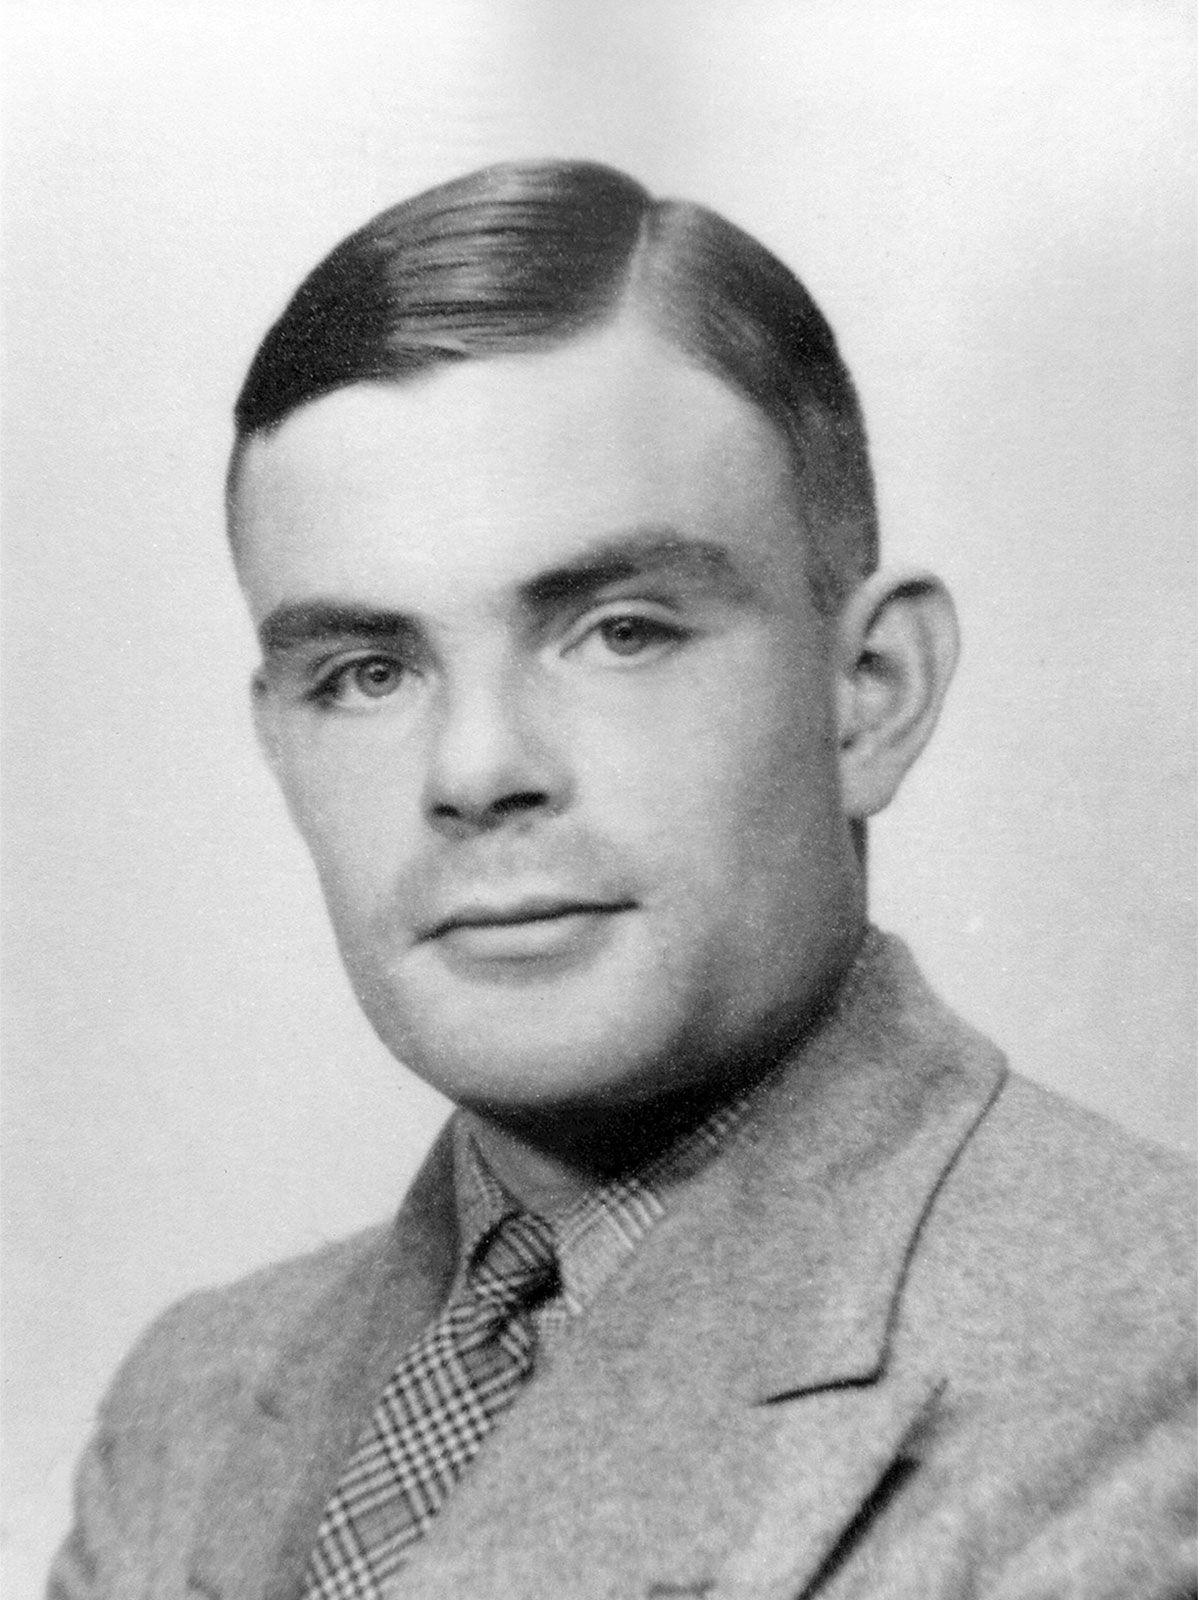
\includegraphics[height=0.75\textheight]{../../assets/Alan-Turing.jpg} \\
                \vspace{0.2cm}
                \textbf{Alan Turing} \\
                \small (1912 -- 1954)
            \end{center}
        \end{column}
        \begin{column}{0.6\textwidth}
            \vspace{0.5cm}
            \Large \textbf{La Corporización del Límite}
            
            \vspace{0.4cm}
            \normalsize
            Matemático británico que tomó el límite abstracto de Gödel y lo transformó en un modelo físico-conceptual: la \textbf{Máquina de Turing}. Demostró que el abismo de la incompletitud tiene una manifestación mecánica inevitable.
        \end{column}
    \end{columns}
\end{frame}

\begin{frame}{El Problema de la Parada (\textit{Halting Problem})}
    \begin{center}
        \Large \textbf{El Límite del Algoritmo}
        
        \vspace{0.6cm}
        \normalsize
        No existe ningún algoritmo general capaz de determinar si un programa informático arbitrario se detendrá o se ciclará indefinidamente bajo una entrada dada.
    \end{center}
    
    \vspace{0.6cm}
    \alert{\textbf{La Máquina Destructora ($D$):}} \\
    Si asumes que existe un predictor perfecto ($H$), puedes programar una máquina $D$ que consulte a $H$ y \textbf{haga exactamente lo contrario}. Al evaluar $D(D)$, el universo lógico colapsa en contradicción.
\end{frame}

% ==========================================
% EL HILO ROJO
% ==========================================

\begin{frame}{El Hilo Rojo: La Diagonalización}
    \begin{center}
        \Large \textbf{La topología del límite absoluto}
        
        \vspace{0.5cm}
        \normalsize
        Existe una única firma matemática detrás del infinito de Cantor, la incompletitud de Gödel y la indecidibilidad de Turing.
        
        \vspace{0.6cm}
        \huge
        $$\forall f: A \to \mathcal{P}(A), \quad \exists S = \{ x \in A \mid x \notin f(x) \}$$
    \end{center}
    
    \vspace{0.6cm}
    \normalsize
    \alert{\textbf{El Judo Metamatemático:}} \\
    Tomar las propias fuerzas y reglas de un sistema absoluto y utilizarlas para generar un arma que apunte directamente a su cabeza.
\end{frame}

\end{document}
